\documentclass{article}


\usepackage{arxiv}
\usepackage[utf8]{inputenc} % allow utf-8 input
\usepackage[T1]{fontenc}    % use 8-bit T1 fonts
\usepackage{hyperref}       % hyperlinks
\usepackage{url}            % simple URL typesetting
\usepackage{booktabs}       % professional-quality tables
\usepackage{amsfonts}       % blackboard math symbols
\usepackage{nicefrac}       % compact symbols for 1/2, etc.
\usepackage{microtype}      % microtypography
\usepackage{listings}
\usepackage{graphicx}
\usepackage{subcaption}
\usepackage{color}
\usepackage[svgnames]{xcolor}

\newcommand{\code}[1]{\mbox{\lstinline{#1}}}
\lstset{frame=tb,
escapeinside={(*@}{@*)},
language=Java,
alsolanguage=Python,
aboveskip=3mm,
belowskip=3mm,
showstringspaces=false,
columns=flexible,
basicstyle={\small\ttfamily},
numbers=left,
numberstyle=\color{gray},
keywordstyle=\color{blue},
commentstyle=\color{green},
stringstyle=\color{mauve},
breaklines=true,
breakatwhitespace=true,
tabsize=3,
upquote=true
}

\title{Loop Programming techniques and How it can improve Quicksort Algorithm}


\author{Shoupu Wan \\
\texttt{wanshoupu@gmail.com} \\
}

\begin{document}
    \maketitle

    \begin{abstract}
        Quicksort is one of the pivotal sorting algorithm widely used by modern software.
        Among the quicksort algorithms, there are two main variants---that designed
        by Tony Hoare and by Nico Lomuto, respectively.
        Hoare's quicksort scheme generally has robust and optimal performance but its
        implementation has been quite involved.
        Lomuto's scheme is easier to follow and implementation is less tricky.
        However for certain edge cases its performance suffers a lot.
        In this article, we present useful techniques for programming loops.
        We will show that these techniques can be used to improve the implementation of quicksort
        algorithm such that it
        has both the robust performance of Hoare's scheme while and the
        succinctness implementation of Lomuto's.
    \end{abstract}


    % keywords can be removed
    \keywords{Quicksort \and Loop rotation \and Nested loop compression \and Cascading conditional
    \and Sentinel}


    \section{Introduction}\label{sec:introduction}
    As one of the most widely used programming constructs, loop is productivity
    amplifier and is featured in almost all programming languages.
    With a static body and nominal overheads (\textit{e.g.},
    state-registering variables, \textit{etc.}), a loop can be executed as many times as desired.


    A key building block as loop is, it is worth every developer's effort to master the best
    practices of it.
    On the opposite, it is not uncommon to spot in production code, especially algorithm-intensive
    code haphazardly constructed loops, often with duplicate code dangling around.
    Obviously developers who authored the haphazardly `working' code were either oblivious
    with good programming practices or does not bother to spend the time on better loop constructs.

    Common problems programmers tend to make while programming with loops are
    \begin{enumerate}
        \item Duplicate code between initialization and loop body
        or between loop body and post-loop processing logic
        \item Nested loops
        \item Leaky loop variables
        \item Heavy-duty initialization
    \end{enumerate}

    Duplicate code is the foremost problem in loop programming
    and is among the top root causes for bugs.
    Duplicate code anywhere is bad.
    But duplicate code in and around loops is hard to realize and even harder to get rid of.


    The next commonly held misunderstanding about loop is the tendency to use nested loops.
    Many are ready to jump to the argument about this: ``What's wrong with nested loop?''
    The use of nested loops in many occasions seems to be necessary, reasonable,
    and at least harmless at first sight.
    But this belief stands only at the first sight.
    For almost all cases, nested loops bring complexity rather than convenience, obstruct
    readability rather than facilitating it, deepen the coupling rather than reducing it,
    and discourage code reusability rather than encouraging it.


    The third controversial usage of loops is exposing loop variables to subsequent programming
    units.
    This is essentially passing information from loop to subsequent programming units via the
    exposed variable(s) in an implicit way.
    The problem of this practice is that this expose the implementation details to subsequent
    program and it violates the encapsulation principle.


    Finally the fourth problem with loop programming has to do with disproportionally heavy-duty
    initialization.
    Many programmers prepare for the ensuing loop with a multi-line `min-program'.
    Some are so aware of this problem that they factor out this portion of code into a
    separate function.
    But more often than not, the initialization can be done with a one-liner in a much simpler
    form.


    In this paper we are not going to address all these problems.
    Instead, we will focus on two of them---duplicate code and nested loops.
    Accordingly, we will introduce two techniques---`loop rotation' and `Nested loop thinning'.
    These are the two pillars for loop programming.
    Proper use of them help developers avoid commonly made mistakes.


    As an illustration and proof of the effectiveness of these techniques, we will conduct
    a case study about the well-known quicksort algorithm.
    First invented in 1960, quicksort has been studied and analyzed well over the
    years\cite{Hoare1961,Hoare1962,Sedgewick1978,Bentley:1986:PP}.
    As a `divide-n-conquer` algorithm, quicksort has a profound influence over programming.
    So much so that quicksort is named one of the top $10$ algorithms of $20$th
    century\cite{top10algorithm:2000}.
    For its expected high performance, quicksort becomes the \textit{de facto} sorting algorithm in
    practice.
    By applying these programming techniques, we will present a new and simpler way to implement
    Hoare's quicksort algorithm.

    In what follows, I am going to present the idea in Python 2.7.


    \section{Loop Rotation}\label{sec:LoopDesignConsideration}
    \begin{figure}[htb]
        \centering
        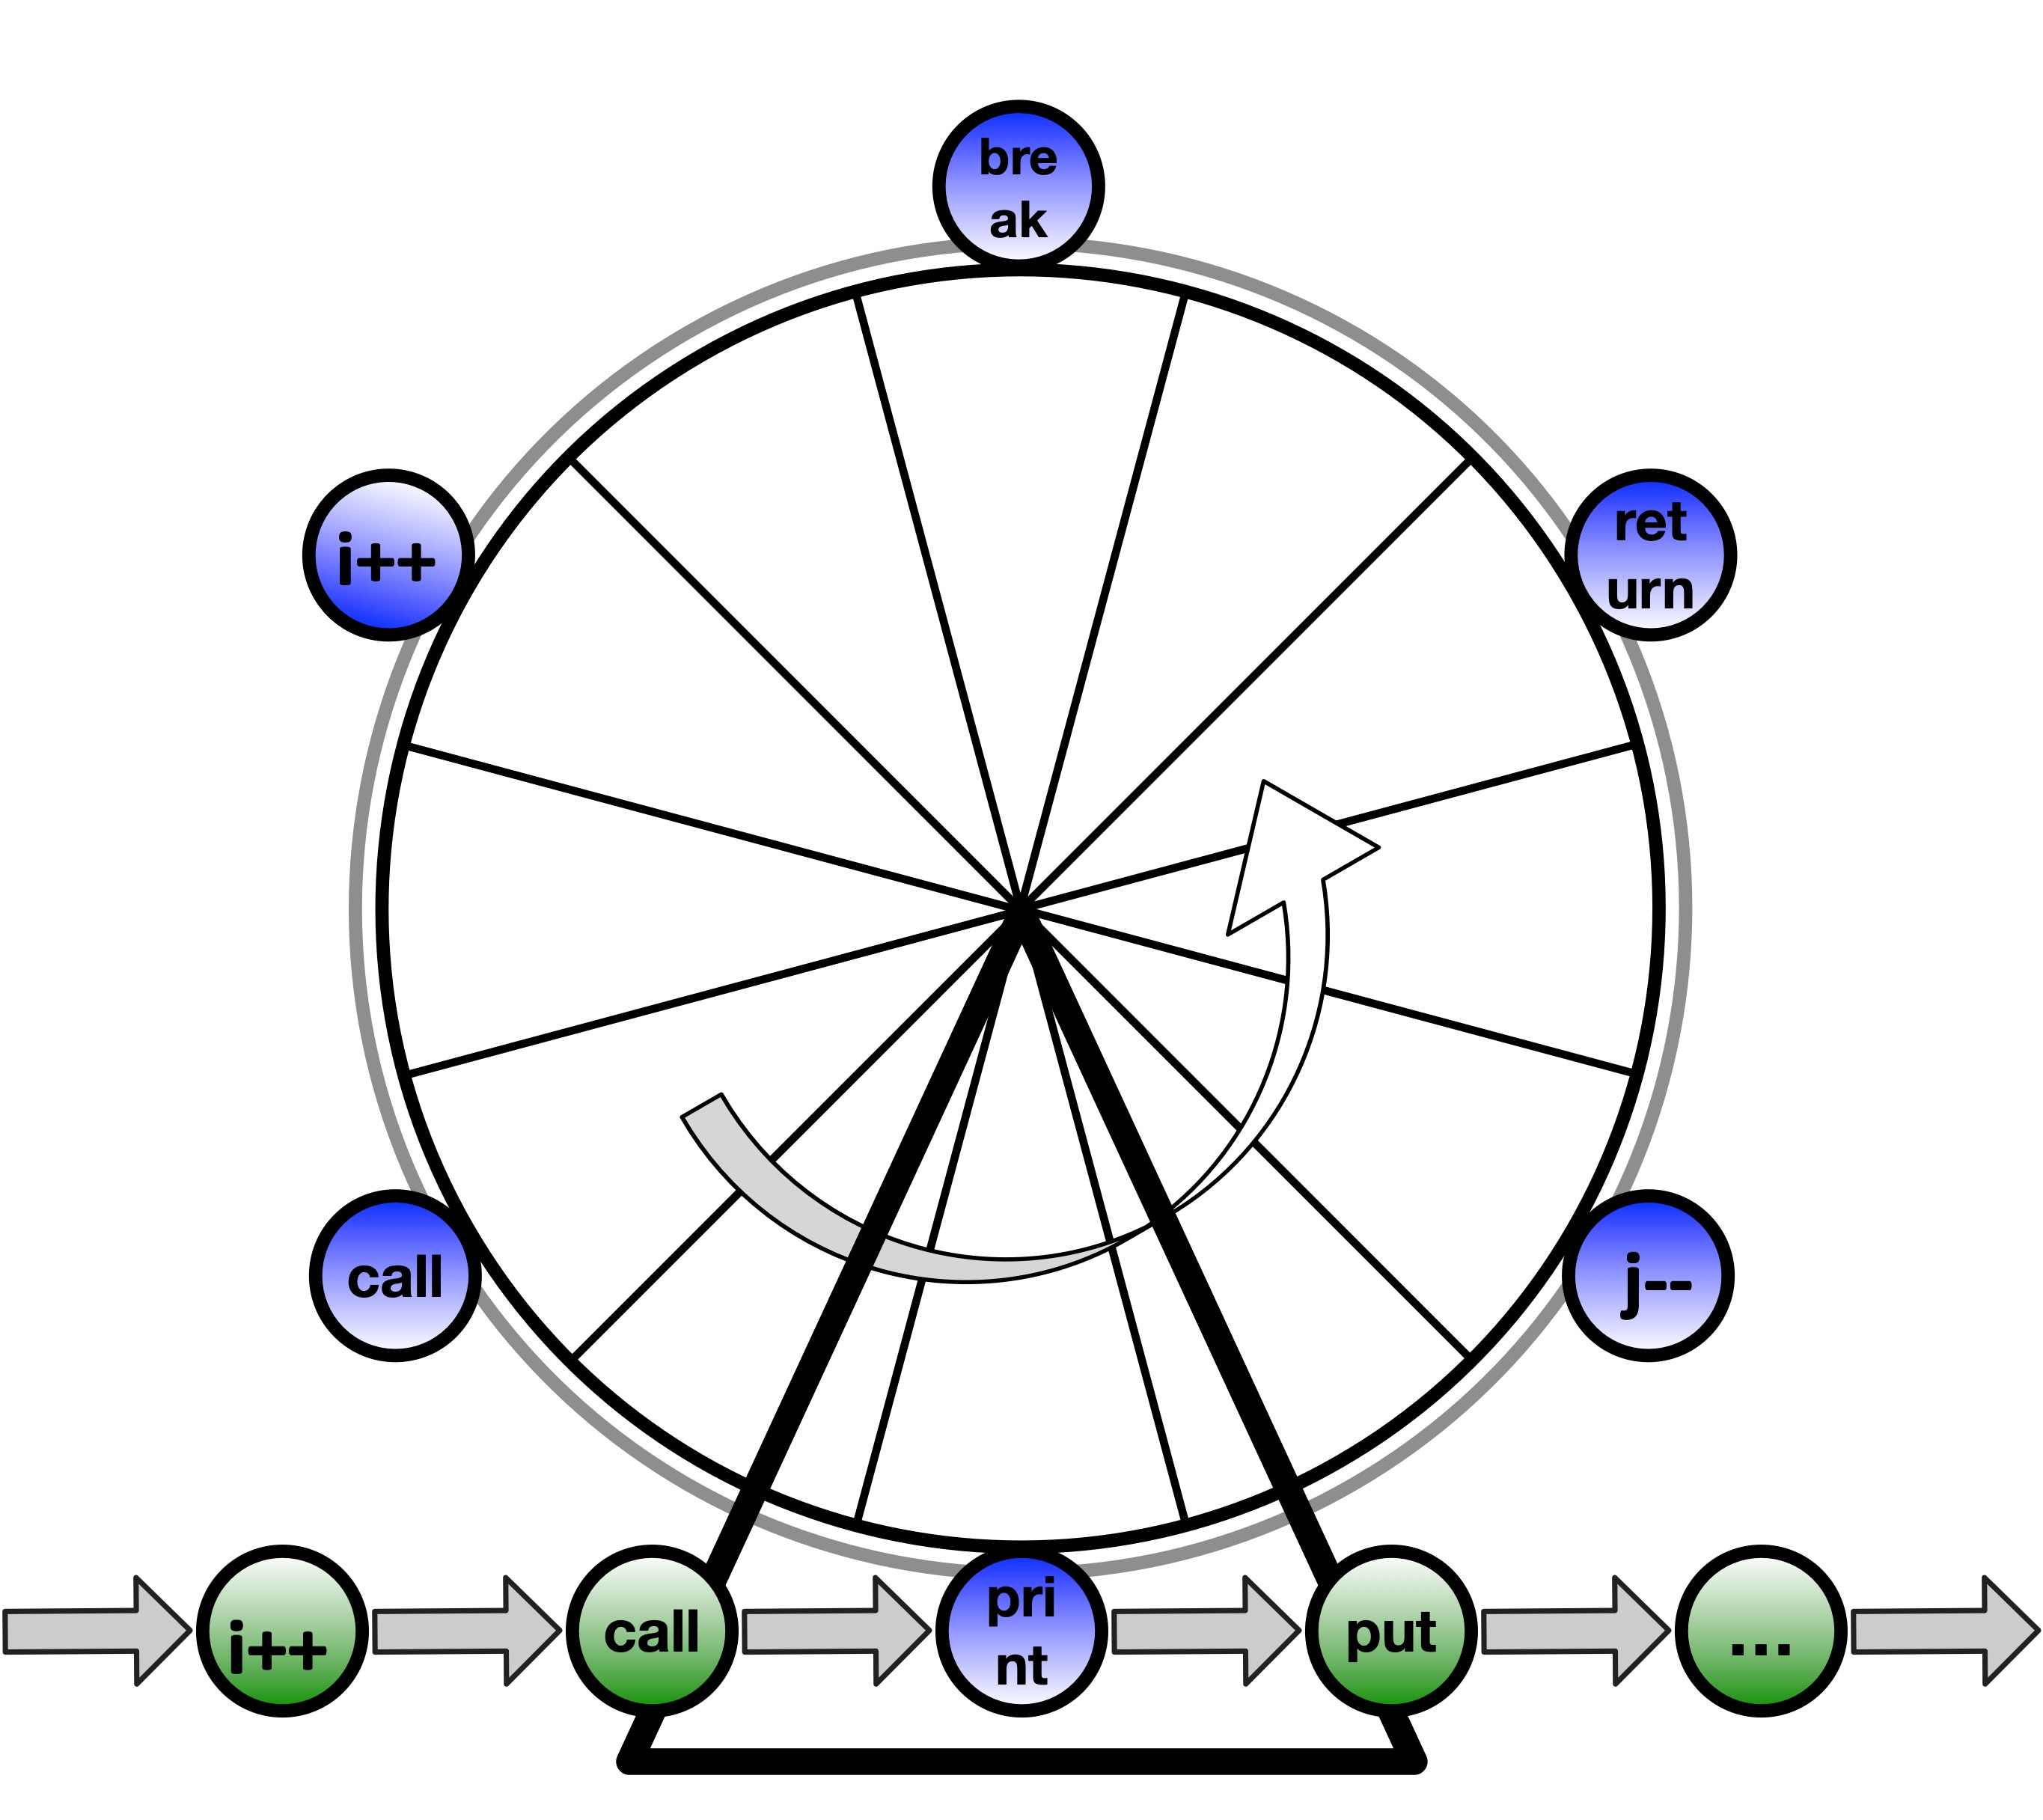
\includegraphics[width=.7\textwidth]{ferris-wheel.jpg}
        \caption{\label{fig:loop-rotation}Loop as a circular sequence.
        The nodes \code{i++} and \code{print} are candidates that can matched and coalesced into
        the loop.}
    \end{figure}


    The key to program loops is to observe two characteristics of them.
    First, a loop construct contains many moving parts and they are tightly
    coupled---changes in one necessitate changes in several others.
    Secondly, a loop does not live in vacuum---it must get along with other code in the vicinity.
    As a result, a large part of the work is spent on fitting loop in the program.


    The biggest problem with loop programming is duplicate code in and around the loop.
    The foremost goal when implementing loop is to reduce duplicate code and
    an important technique for this is `loop rotation'.


    It is beneficial to visualize a loop construct as a Ferris wheel, a carousel, or a spool.
    A property is shared by them all---they can be mathematically represented by circular sequences,
    that is, a sequence with rotational symmetry with respect to circular shifts.


    For sake of argument, in ~\autoref{fig:loop-rotation} we pictured a loop as a Ferris wheel.
    Distributed around the wheel are the loop statements---initialization,
    loop test, state-updating statements \textit{etc.}


    \begin{figure}[htb]
        \centering
        \begin{subfigure}{.45\textwidth}
            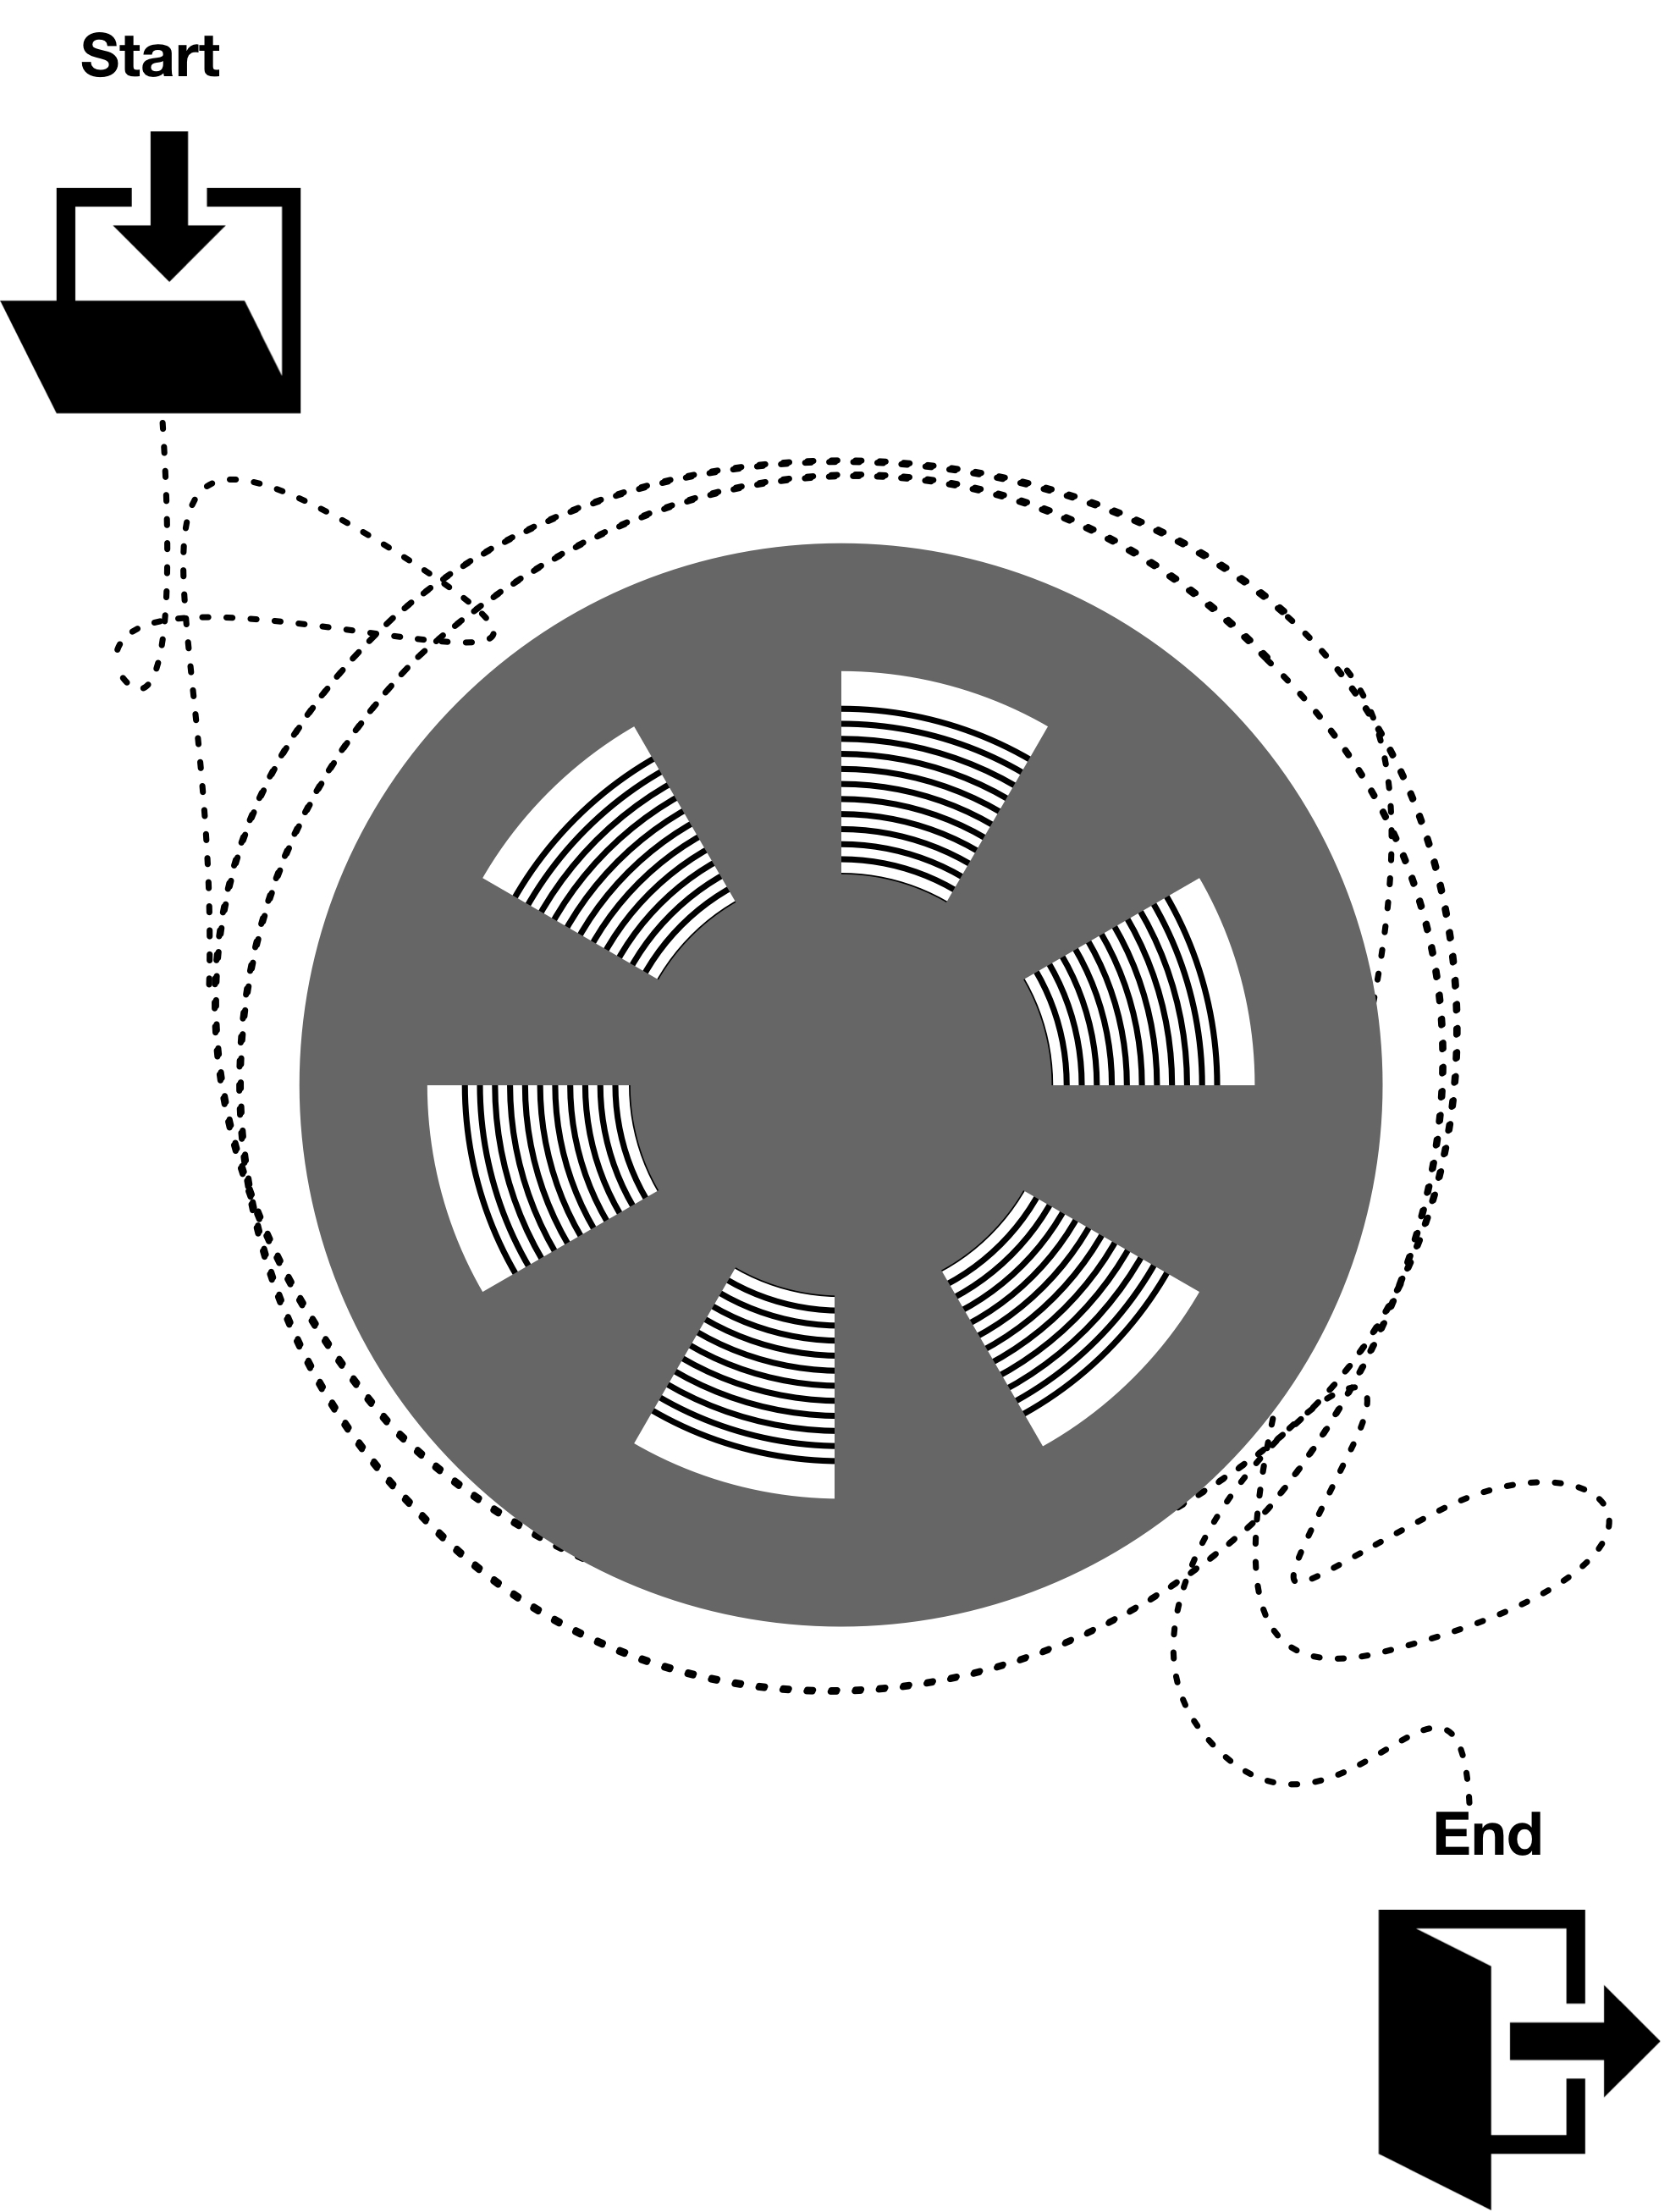
\includegraphics[width=\textwidth]{loose-spool.jpg}
            \caption{\label{fig:loose-spool}}
        \end{subfigure}
        \begin{subfigure}{.45\textwidth}
            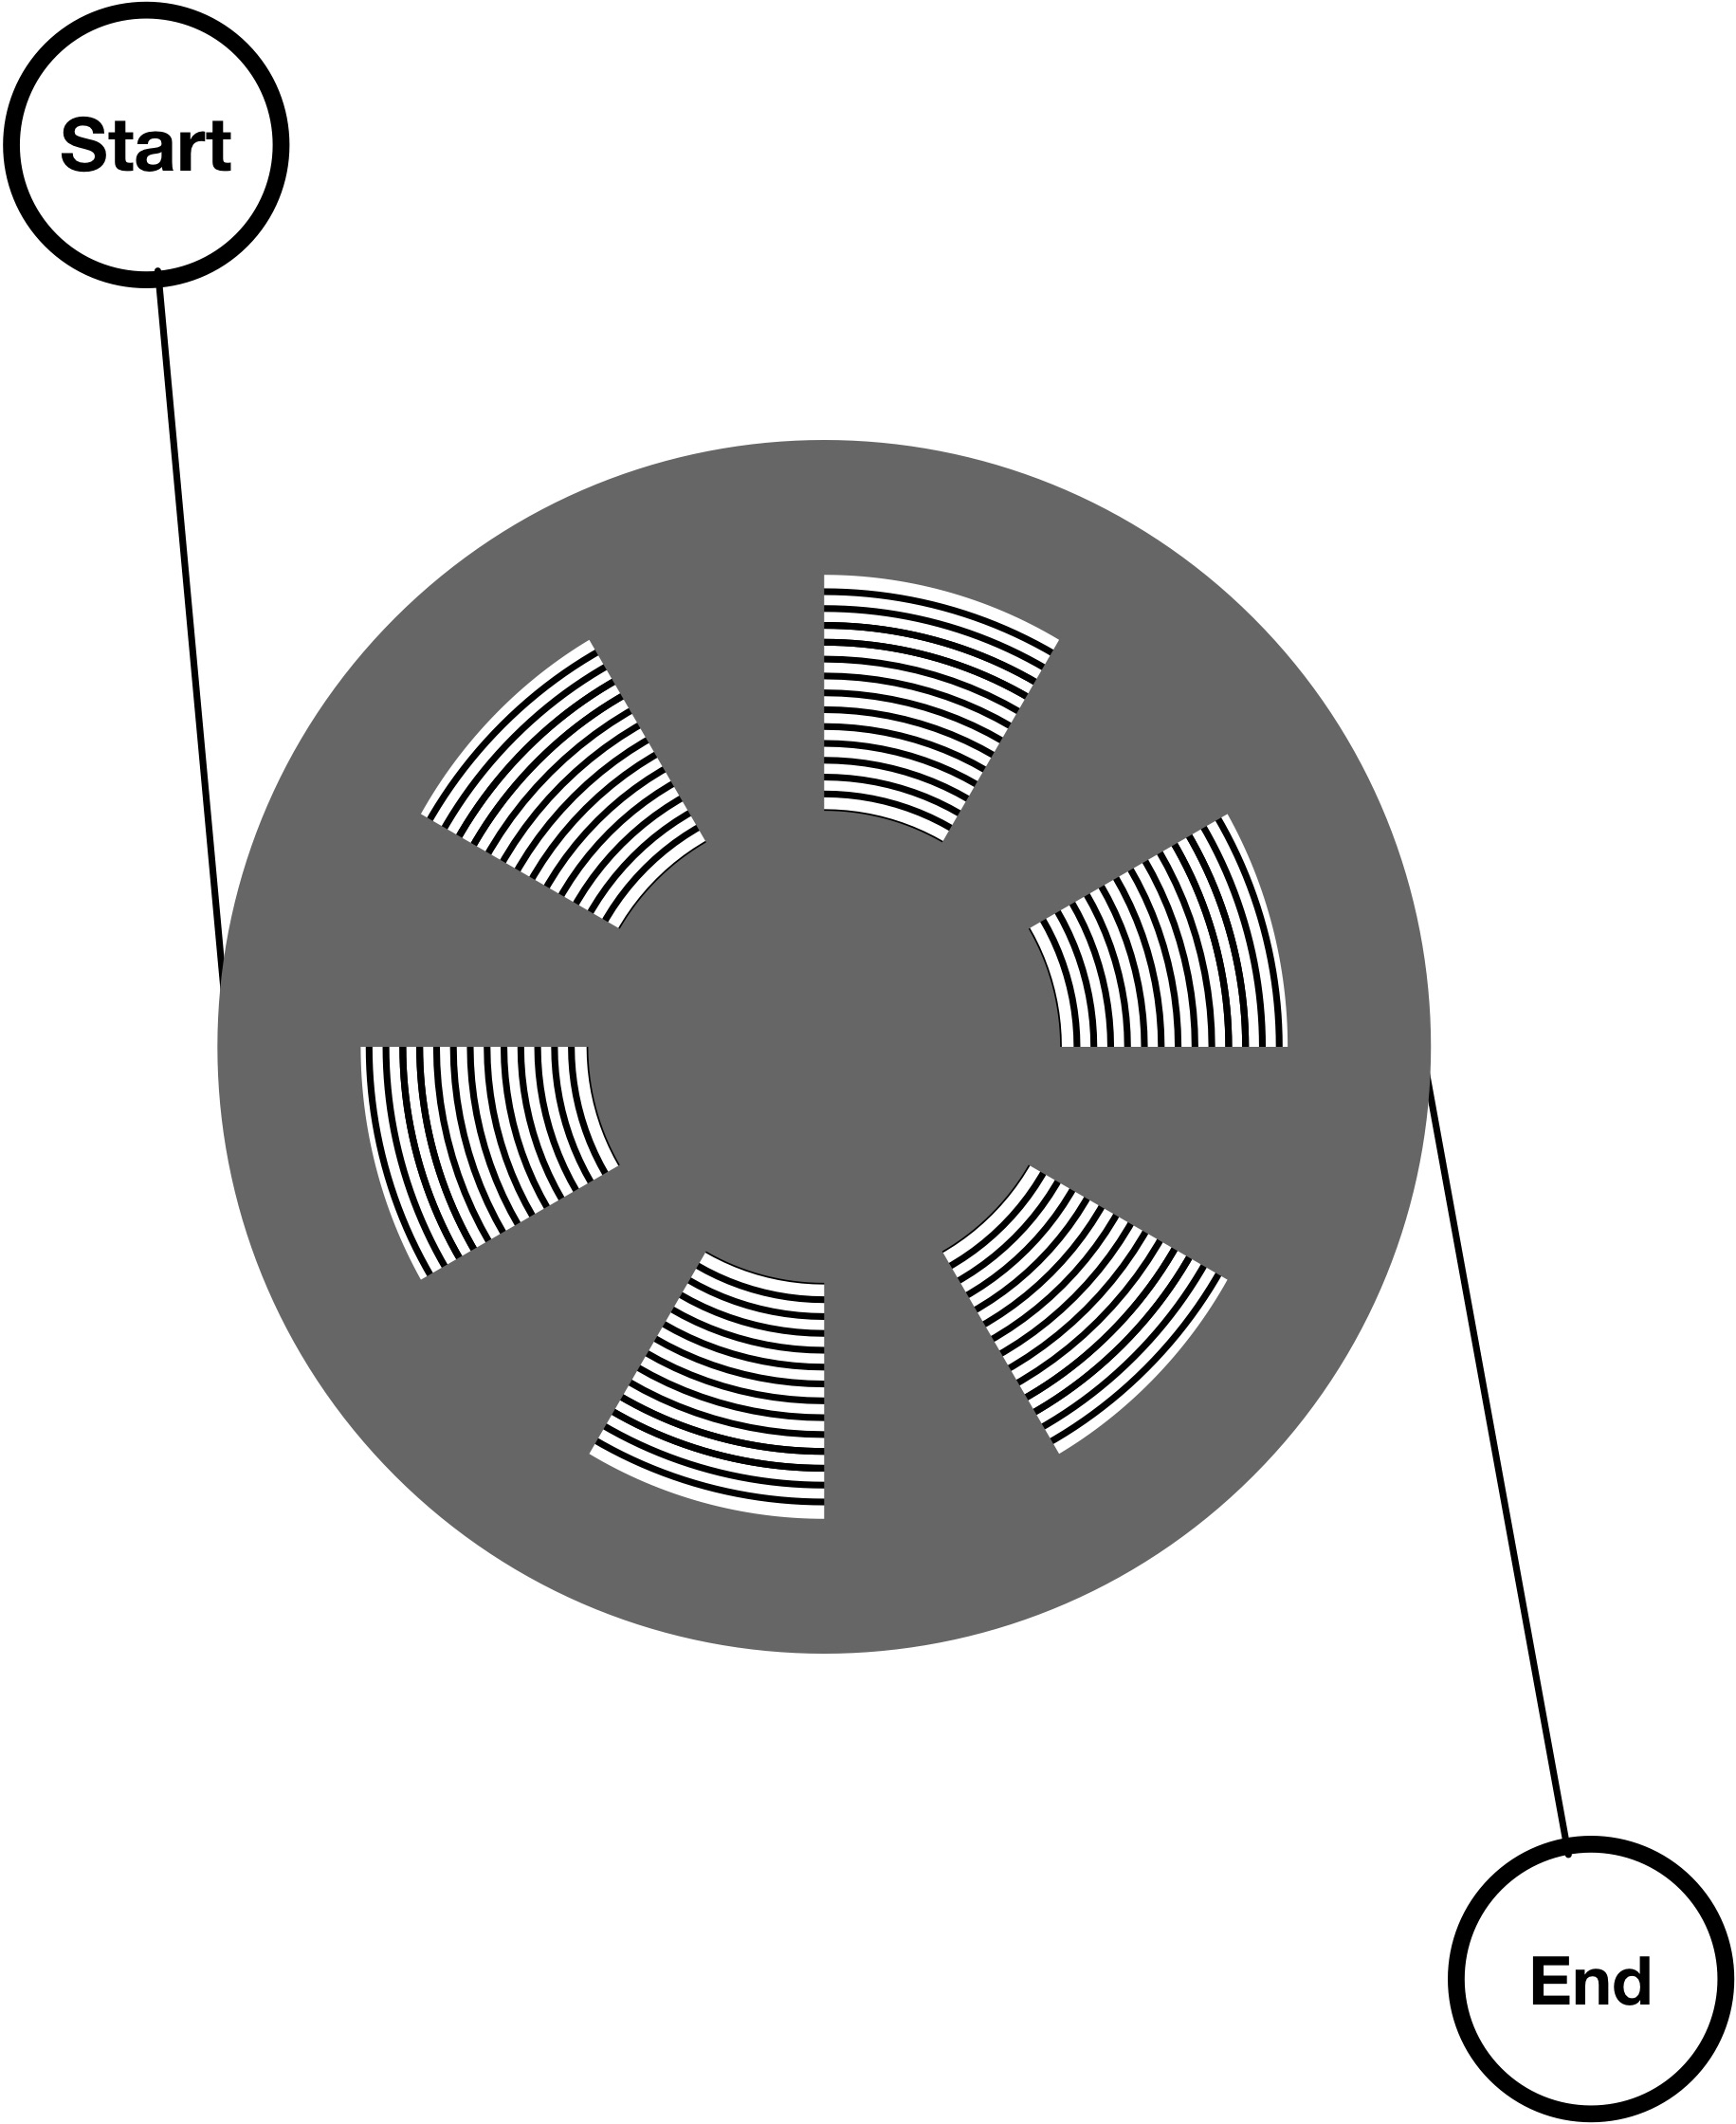
\includegraphics[width=\textwidth]{tight-spool.jpg}
            \caption{\label{fig:tight-spool}}
        \end{subfigure}
        \caption{\label{fig:spool-loop} Using spool as a metaphor for loop in program,
        duplicate code around a loop would be like tightening messy yarns into neat spool.
        `Loop rotation' can be pictorially depicted as winding up loose yarns onto a spool.
        \protect\subref{fig:loose-spool}: Duplicate, sloppy code is analogous to loose, unorganized
        yarn around a spool.
        \protect\subref{fig:tight-spool}: A neat loop is analogous to a tidy spool.}
    \end{figure}


    As another helpful analogy, loops are to program as spools are to yarn.
    In the same way as a spool is used to organize yarn, a loop is a construct to organize program.
    From this perspective, the `loop rotation' process to coalesce duplicate code is analogous to
    wind up loose, messy yarn into a tidy spool (~\autoref{fig:spool-loop}).


    Even though a loop is a circular sequence, there is always an entrance and an exit.
    One can thus take this rotational degrees of freedom to one's advantage as to determine where
    to enter and where to exit the loop.
    For example, if the code in the loop and in the affinity of the loop are duplicate, one may
    `rotate' the loop to match up and coalesce the duplicate code.
    On the contrary, if one wants to move a portion of code at the beginning of the loop out of
    the way, one may `rotate' the loop in the reversely.
    Doing so may result in duplicate code, but this may enable a subsequent refactor whose
    positive effect will eventually pay off this adverse effect.
    In general, we will refer to this loop fine-tuning programming technique as `loop rotation'.


    In practice, one may first implement a prototype with unconditional \code{while (true)} or
    \code{for (; ;)} loop.
    This will push all the statements into the loop body for ease of `loop rotation'.
    This will help one focus on coming up with \emph{a} `working' code first.
    Once a `working' code has been found, one can use the `loop rotation' technique to fine-tune
    the program.


    For `soft' code duplication---two blocks of code that are not
    identical but share certain pattern, one may perform pre-refactor to
    consolidate the `shared duplication' into copy-n-paste duplication and then treat the
    duplication in the normal way.


    \section{Nested Loop thinning Technique}\label{sec:loop-thinning-technique}

    Every developer writes nested loops now and then.
    Many times, nested loops appear compelling and inevitable.
    While they may solve our problem, nested loops inflate a program with
    unnecessary complexity.
    Nested loops, with the extra layers of loop gadgets, also obstruct code readability.
    The presence of nested loops usually conceal numerous optimization opportunities.

    Great developers will try best to reduce the layer of loops, even avoid using loops
    altogether with certain programming language or software framework especially for scientific
    computation and data engineering\cite{data-engineering-avoid-loop}.
    The removal of nested loops often results more optimizations obvious and
    accessible.
    Like `Candy Crush Saga' game arriving at a critical point, a single move may unlock an
    avalanche of moves, to the player's advantage.


    Here we are to present a process that coalesce nested loops into a single loop,
    known as `nested loop thinning' technique.
    Cramming all the functionalities of nested loops into one loop is hard by definition.
    As a price to be paid, `nested loop thinning' process almost always
    results in one or more of these changes to the final loop:
    \begin{itemize}
        \item extra conditional constructs are added
        \item extra tests are added to existing conditional constructs
        \item the pacing of the resulting loop is made more dynamic
        \item more boundary condition handling logic is added
        \item auxiliary data structure, such as queue or stack, is added.
    \end{itemize}


    \begin{figure}
        \centering
        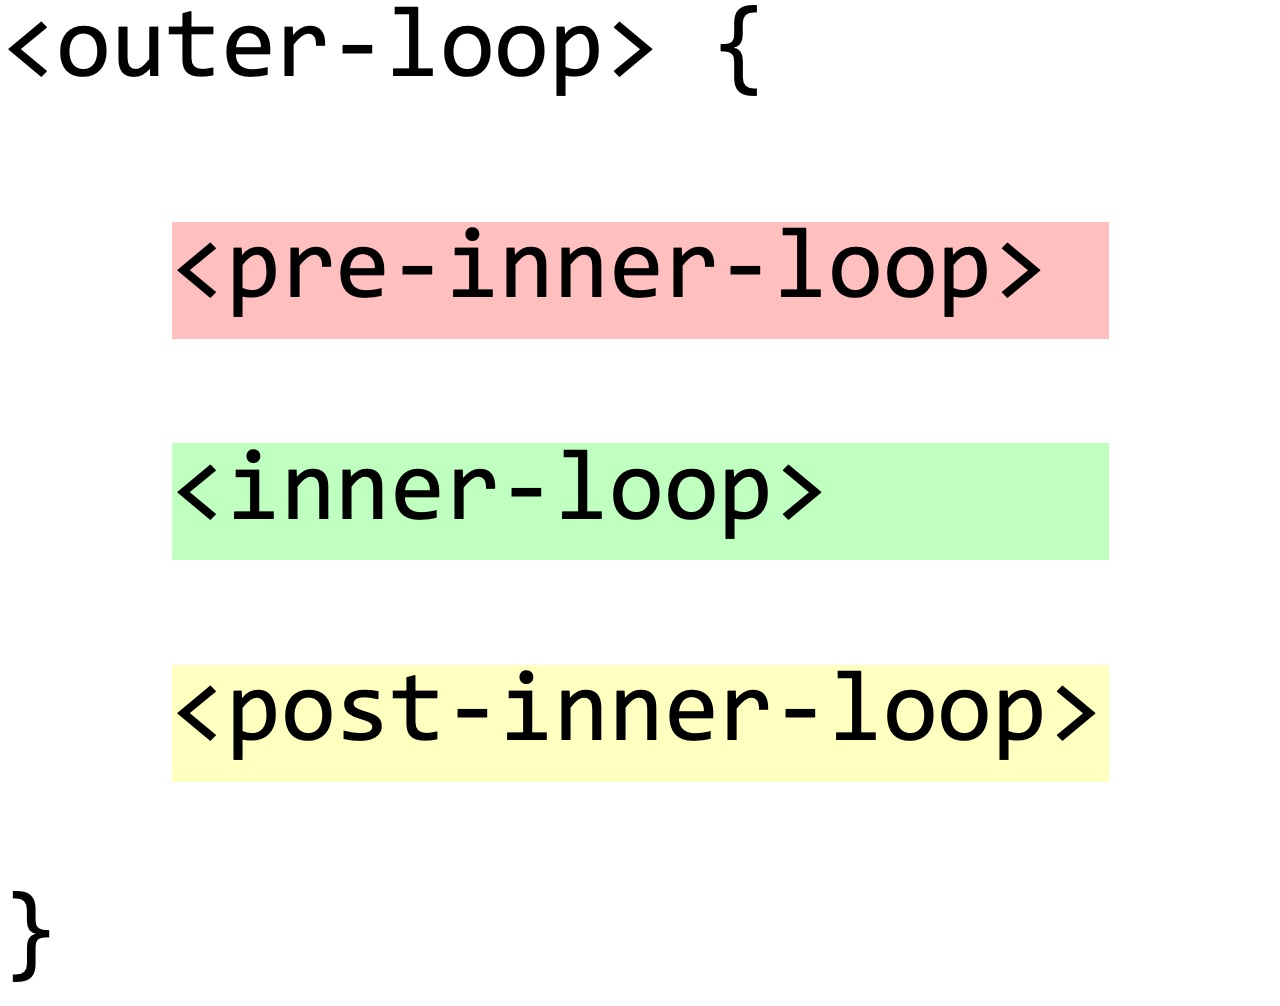
\includegraphics[width=0.6\textwidth]{segment-for-loop-thinning.jpg}
        \caption{\label{fig:segment-for-loop-thinning}
        Sectioning of loop body statements for `nested loop thinning' process.
        Each section receives different treatment during the `nested loop thinning' process.}
    \end{figure}
    For sake of argument, the body of the outer loop is
    divided into three sections---\emph{pre-inner-loop} section, \emph{inner-loop} section, and
    \emph{post-inner-loop} section---depending on their relative position
    in respect to the inner loop (shown in ~\autoref{fig:segment-for-loop-thinning}).


    The gist for flattening nested loops is as follows.
    First, we need to move pre-loop statements out of the way.
    To that end, use `loop rotation' technique (see ~\autoref{ch:loops}) backward
    to unwind the pre-loop statements.
    The second step depends on the inner loop construct.
    If the inner loop has a \emph{non-trivial loop condition}, then the inner loop can
    be converted to a conditional construct as-is by keyword swapping: \code{while} $\rightarrow$
    \code{if}.
    At the same time, the post-inner-loop statements shall be wrapped away in a piggybacking
    \code{else}-clause.
    On the contrary, if the inner loop is \emph{unconditional}, chances are that
    there is a conditional \code{break} statement somewhere in the loop body.
    Then one can tuck the post-inner-loop statements under the conditional of the
    \code{break} statement replacing the latter, and the inner loop can be stripped away.


    Throughout the process, one shall pay special attention to execution-path altering statements,
    such as \code{break} and \code{continue}.
    Regardless the venue taken, new conditional statements are inevitably formed and cascading
    conditional constructs are the best way to organize them.
    one may refer to Reference ~\cite{Wan:book} for best practices on how to organize effective
    cascading conditionals.


    Apart from the prescribed steps, some preparatory measures may be taken beforehand
    to reduce the friction during the `nested loop thinning' refactor process.
    Where needed, compound statements may be taken apart before one wades deep.
    Compound statements may get in your way of refactoring for multiple reasons.
    The most obvious reason is that, well, parts of a compound statement
    may end up at different places after refactoring.
    Non-idempotent conditional expressions, such as \code{if (--i < 0)}, are even more lethal
    because each execution of the condition ratchets the state of the loop, leaving no time for
    taking a breath.
    For example,
    \begin{lstlisting}
        while (++i < LIMIT);
    \end{lstlisting}
    shall be expanded to
    \lstinputlisting[]{expanded-do-while.java}
    before the start of loop thinning refactor.
    The following Golang statement should also be unfolded beforehand:
    \begin{lstlisting}
        if v := a[i]; v < LIMIT
    \end{lstlisting}


    In the `nested loop thinning' process, as one can
    simply replace the keyword \code{while} with \code{if} when due.
    Therefore, \code{while}-loop readily lends itself to this refactor process.
    For this reasons, \code{for}-loop with all its header statements, should be taken apart and
    converted to \code{while}-loop during the preparation stage.


    After `nested loop thinning',
    cleanup changes may be performed to comply with convention, code style, or purely for
    cosmetic reasons.


    There are application restrictions of the `nested loop thinning' process.
    Firstly, inner loop must be directly embedded in outer loop with no intermediate layers.
    Also execution-path-altering statements, such as \code{break}, shall be absent in the
    pre-inner-loop section.


    Most of the methods we present in this article are empirical, the author does not claim
    universal applicability for many of them.
    Instead, the techniques shall be considered on a case by case basis.

    One particular case whose success is almost guaranteed is a type of nested loops where
    the outer loop represents an evenly-paced, end-to-end iteration over a data structure whereas
    on the inner loop is performed a lookup on an auxiliary data structure or
    a `sliced view' of the same data structure.

    In what follows, we are going to demonstrate application of `nested loop thinning' technique
    on the quicksort algorithms.
    Through the application of this refactor process, %TODO


    \section{Case Study: quicksort}\label{sec:nested-loop-quick-sort}

    We will now consider another case study.
    This is a classical example that was detailed by books such as `Programming
    Pearls' and `Numerical Recipes'\cite{Bentley:1986:PP, NumericalRecipes:1992}.
    My encounter with the code in these books completely redefined the word `simplicity'
    in my dictionary.


    My first implementation of the quicksort algorithm was in C based off
    the traditional ``Hoare's partitioning'' scheme, as presented
    in `Numerical Recipes' (minus the sentinel part).
    But in what follows, I am going to present the idea in Python 2.7.


    The outline of the quicksort function is as follows.
    \lstinputlisting[label={lst:QuickSortOutline},language=C,
    caption={An implementation of quicksort algorithm.}]
    {quicksort_outline.c}
    where arguments \code{s} and \code{e} are the starting (inclusive) and ending (exclusive) pointers
    to the array.
    `\code{part}' is a recursive function whose base case is no-op, namely,
    arrays with fewer than two elements.
    With a pivot element randomly chosen out of the array,
    a large array is partitioned into three consecutive parts: the pivot element in the middle, a
    subarray on the left, and a subarray on the right.
    Then the pivot element is swapped into its final position.
    After this, each of the two subarrays is subject to the same function.
    So on and so forth until each subarray is reduced to the base case.
    At the return of the first call of the function, the entire array is left in sorted state.


    As you may have noted, we emphasise that the partitioning function divides an array into three, not
    two, parts---the pivot element $p$, the partition $\leq p$, and the partition $\leq p$.
    This is crucial to the convergence / termination of the function.
    It may be the case that one or the other of the two partitions is empty.
    But even so, please remember the partitioning scheme employed in quicksort is \emph{three-way}.


    With the Hoare's partitioning scheme, a tentative implementation for the function \code{part} is as
    follows.
    \lstinputlisting[label={lst:nestedLoopHoareMethod},language=C,
    caption={Implementation of Hoare's partition scheme for quicksort.}]
    {quicksort_partition_sym.c}
    First, we randomly select a pivot element and swap it to the beginning of the array
    (ask yourself: ``why beginning of array?
    Why not end?'').
    Then two pointers, \code{s} and \code{e}, starting off the opposite ends of the array,
    wade toward each other.
    Each of them makes stop at `out-of-place' element.
    When both stop, that is when a pair of `out-of-place' elements have been discovered,
    a swap is performed to bring both elements to the respective partitions they belong to.
    Then the pointers are back on their way toward each other once again.
    So on and so forth until they meet or cross.
    At that point, the pivot element (at the beginning of the array) is swapped into its final position.
    Finally, a pointer pointing to this position is returned.


    The above visual description of Hoare's partitioning scheme disguises the true complexity of
    implementing it.
    %unexpectedly tricky to implement.
    so much so that once in a while when my memory of any previous implementations becomes blurry or
    totally fades away, it may take me quite a few days to implement a solution that can pass a
    handful of unwitty test cases.
    Thus repeated several times, I decided to summary the frequently-made bugs and produced a list of
    `gotcha' as follows:
    \begin{enumerate}
        \item In pivot election, failure to swap pivot element to the beginning of array
        \item For the pointers \code{s} and \code{e}, there are two hesitating options:
        `check-then-increment' or `increment-then-check'.
        The first option leads to infinite loop for certain cases.
        \item Also a choice between `\code{<= pivot}' and `\code{< pivot}' for \code{s},
        `\code{>= pivot}' and `\code{> pivot}' for \code{e}.
        Incorrect choice may inadvertently cause pointer incrementation to be skipped under
        obscure circumstances which will, in turn, cause infinite loop
        (Remember that under no circumstances, should either pointer stops approaching each other in
        any outer loop iteration before they meet or cross.)
        \item\label{itm:quicksort-boundary-condition} In the second inner loop for pointer \code{e},
        failing to check boundary condition causes `out-of-boundary' exception.
        Incorrect boundary condition, such as \code{s < e}, again cause pointer \code{e} to stall
        in the middle of the right partition.
        This will cause the pivot is placed at the wrong place at the return of function.
        \item Outer loop termination logic also needs deliberation.
        The key decision to make is `where to break or return' rather than `when to break or return'.
        For ~\autoref{lst:nestedLoopHoareMethod}, the choice of location of return
        at the end of the loop body was made after quick a few failed attempts.
        \item Fail to swap the pivot element to its final position.
        This step often poses a stumbling block for beginners as well as other unsuspecting
        developers.
    \end{enumerate}
    In fact just to debug ~\autoref{itm:quicksort-boundary-condition} and
    figure out the correct condition \code{pivot < e}, instead of \code{s < e}, took me $2$ good hours.
    Also, deciding out the semantics of the function arguments in `\code{qsort}' took me
    quite some deliberation before I finally got them right.


    A large part of the complication of the problem comes from the fact that this implementation
    consists of many parts that are highly entangled---changing one would necessitate simultaneously
    changing others.
    For example,
    %the return value of the partition function is picked among .
    suppose we are going to change the semantics of \code{e} from exclusive to inclusive, what
    would the pointer to be returned change to?
    \code{s}? \code{s+1}? \code{e}? Or \code{e-1}?
    Accompanying these changes, the recursive calls
    \begin{lstlisting}
        qSort(s, p);
        qSort(p + 1, e);
    \end{lstlisting}
    also need changes.
    With the choice of return value, should the recursive calls be changed to
    \begin{lstlisting}
        qsort(s, p - 1)
        qsort(p + 1, e)
    \end{lstlisting}
    or
    \begin{lstlisting}
        qsort(s, p + 1);
        qsort(p + 2, e);
    \end{lstlisting}
    or some other form?
    The number of combinations for such changes grows exponentially as the degree of coupling increases.


    This partially explains why it is so hard to correctly implement this seemingly simple partitioning
    function.
    On the one hand, the problem itself is complicated---the number of loose parts exceeds what our
    brain can comfortably handle at once.
    On the other, however, the way we approach the problem makes it harder---it is all because
    we attempted to fight too many wars all at once.
    The complexity of the problem is doubled, or tripled, the moment we decide to send one pointer
    from each end of the array to meet somewhere in the middle.


    Is there a more straightforward way to implement the quicksort algorithm?
    Yes!
    There is a simpler and more compact partition scheme credited to Nico Lomuto\cite{Bentley:1986:PP}.
    By sending two pointers off the same end of the array, the Lomuto's partitioning scheme
    successfully avoids fighting two frontiers at the same time and thus greatly simplifies the
    partitioning process.


    The two pointers each has a distinct task, each on its own pace.
    The one running in front, so-named `frontier', is responsible to discover out-of-place elements.
    The one running behind, aka, `guardian', guards the partition boundary.
    When the frontier discovers an out-of-place element, the guardian pointer is incremented to make
    room for it and a swap places it there.
    Finally, the pivot element is swapped at the boundary place.
    Notably, implementing this partitioning scheme only needs one loop
    (see blow ~\autoref{lst:singleLoopLomuto}).
    \lstinputlisting[label={lst:singleLoopLomuto},language=C,
    caption={Implementation of Lomuto's partition scheme for quicksort.}]
    {quicksort_partition_asym.c}


    Comparing ~\autoref{lst:nestedLoopHoareMethod} with ~\autoref{lst:nestedLoopHoareMethod},
    one can't help but be surprised ``Seriously?
    A single loop can replace three?''


    Unlike the arduous implementation and debugging process of Hoare's,
    that of the Lumoto's partitioning scheme has fewer moving parts, contains fewer surprises, and is
    easier to follow.
    However there is no free lunch.
    The simplicity of Lumoto's quicksort comes with performance penalty
    for certain cases, with one such case being large arrays with a significant amount of elements
    of the same value.
    In such cases,
    the Lomuto's quicksort scheme tends to degrade to quadratic runtime complexity.
    (Can you figure out why?)
    In comparison, the Hoare's partitioning scheme is stable and
    robust with respect to such cases, always performs at a steady O( N log N) expected runtime.
    %\footnote{The reason is as follows.
    %When faced with equal-valued elements, both ~\autoref{lst:nestedLoopHoareMethod}
    %and ~\autoref{lst:singleLoopLomuto} still do pair-wise swap among two equal elements.
    %But the ending position for the pivot element is seriously off to the right end of the array for
    %Lomuto's partitioning scheme whereas that of the Hoare's ends up at the middle.}.
    For this reason, Lomuto's partitioning scheme is not suitable for general-purpose libraries.


    However, Lomuto's quicksort algorithm is still inspiring for its simplicity and elegance.
    It is tempting to ask: ``Is there a quicksort implementation that has the simplicity of Lomuto's
    \emph{and} the performance of Hoare's?''
    I don't know for sure.
    But with our `nested loop thinning' technique and other tools we developed in the last section
    and this, we
    can explore a little bit to see if we can approach the above goal any closer than the existing
    two schemes.
    %Now that we have the `nested loop thinning' technique in hand, we can take on this challenge for a good
    %cause.
    %The aforementioned loop thinning technique can be used to further simplify the Hoare's partitioning
    %algorithm.
    Our starting point is the Hoare's quicksort implementation of ~\autoref{lst:nestedLoopHoareMethod}.
    As mentioned earlier, the trickiest part of that program is the nested loops which also consists
    of the major complication.
    Let us forcus on getting rid of that.
    %a single-loop with cascade conditionals in the loop body
    %(refer to ~\autoref{ch:conditional-cascade}).


    The immediate difficulty is how to take apart the densely packed conditional construct:
    \begin{lstlisting}
        while(s < e && *++s < *pivot);
        while(pivot < e && *--e > *pivot);
    \end{lstlisting}
    The loop conditions here are unusual and awkward to handle
    because both `\code{++s}' and `\code{--e}' ruthlessly ratchet the loop state forward
    whenever control is passed to this line.
    Namely, each evaluation of the loop condition, even if the condition evaluates to false, the
    pointers `\code{s}' and `\code{e}' are still incremented.
    If we use these conditions as is in the to-be conditional constructs, we would end up in a
    dilemma---when we discover out-of-place elements, we would pass them without swap in the next
    iteration because the program does not leave us any chance for that.


    With the existing programming languages' syntaxes, we have no choice but to break
    up the pre-incremental statements.
    So something must be done to unfold the extraordinary loop conditions to
    ordinary ones before we proceed with the rest of the `nested loop thinning' procedure.
    As we learned in ~\autoref{ch:loops}, these loops may be converted first to
    `\code{do-while} loops' such as
    \lstinputlisting[language=C]{quicksort_inner_loop_do_while.c}
    and the latter are, in turn, converted to `\code{while} loops':
    \lstinputlisting[language=C]{quicksort_inner_loop_while.c}
    After these changes are applied, our the partition function becomes
    \lstinputlisting[language=C]{quicksort_partition_sym_expanded_inner_loop.c}
    You may have noticed that we have floated ~\code{--e} up in front of the first inner loop,
    and this does not affect the correctness as can be verified.
    The solution now seems equally messy, if not more so, as we started.
    However, as you will see, this form will prove useful for the subsequent refactor step---`loop
    rotation'.


    Now we can proceed with the next step
    of loop thinning---move the \emph{pre-inner-loop statements} out of the way.
    (``Loop rotation'' is specified in ~\autoref{sec:LoopDesignConsideration}.)
    After this step, the code becomes:
    \lstinputlisting[language=C]{quicksort_partition_sym_rotated_inner_loop.c}
    We have accelerated the process by tucking the \emph{post-inner-loop statements}
    resulted from the loop rotation to a conditional block.


    Now we are ready with the third and most exciting step---converting inner loops to conditionals.
    Now we encounter a complication that is new to us: we need to covert the second loop to an
    `\code{else if}' clause of the first because the second inner loop is executed only after the first
    exits.
    Our final result is posted below after the conversion to conditional construct:
    \lstinputlisting[label={lst:singleLoopHoarePart},language=C,escapechar=\$,
    caption={Implementation of partition function for Quicksort using one pointer.}]
    {quicksort_partition_single_loop.c}
    Note that we have combined multiple statements into a compound one `~\code{swap(s++, e--)}'.
    %By now we conclude our ``nested loop thinning' refactor process.

    By now,
    we achieved our goal of a quicksort partitioning implementation that has the simplicity of
    Lomuto's and the robust performance of Hoare's.
    In retrospection, we set off to test the hypothetical quest for a simple but performant
    partitioning scheme that comprises the advantages of Lomuto's and Hoare's partitioning scheme.
    Comparing with where we started off ~\autoref{lst:nestedLoopHoareMethod},
    we implemented the Hoare's algorithm with a single loop plus
    cascading conditionals as ~\autoref{lst:singleLoopHoarePart}.
    In the process, we used the `loop rotation' techniques, the `nested loop thinning' techniques,
    and skills concerning the construction of cascading conditionals from earlier sections.
    The new quicksort implementation retains the optimal runtime as Hoare's algorithm but has
    comparable simplicity as that of Lomuto's.
    That's almost too good to be true!
    %If this does not impress you, then you have no feeling.
    While we can make the solution simpler with the use of sentinel, we will leave that discussion to
    next section.
    However there is one change that can provide a little more saving.
    If we change the semantic of ending pointer \code{e} from exclusive to inclusive, the
    pre-increment before the loop (line~\ref{quicksort:pre-increment} of
    ~\autoref{lst:singleLoopHoarePart}) would be unnecessary.


    As a byproduct of going through the detailed refactor
    processes for the cases of this section, I want the reader to have a feeling about software
    development model.
    As we can see the most fruitful software development model, undoubtedly, is to come up with a
    working solution first.
    However shabby, messy, primitive a solution it may be, as long as it can pass a handful of unit
    tests, it will be a great starting point.


    Then through meticulous optimization process, for which many of the techniques we have talked
    about and will be talking may be an aid, strive for straightforwardness, simplicity, and elegance.
    In the course, one may discover new issues, adding new unit tests accordingly, and obtain new
    solutions.
    With the variety of solutions passing the same unit tests, one can often form a better
    perspective regarding the solution space.
    This will help one pick the most effective solution to the original problem.
    %This is as a general programming guideline as well as specific  ally applicable to loops.


    \section{Case Study: quicksort}\label{sec:quick-sort-sentinel}


    I came to learn about sentinels from the book ``Numerical Receipt in C''
    ~\cite{NumericalRecipes:1992} in the section ``Quicksort''.
    It was eye-opening to see how the authors gracefully avoided the array boundary checks
    with the use of sentinels.
    I psychologically accepted the pitch made for sentinels while I was with the book.
    Closing the book, however, I am still dubious about its plausibility until I myself have a
    success implementing it.
    In this section, I pick this work to make a pitch to the reader about sentinels.


    For stark effect of the sentinels, we will first fix the traditional implementation of `Hoare's
    partitioning' scheme:
    ~\autoref{lst:QuickSortOutline} gives the outline of the program and
    ~\autoref{lst:nestedLoopHoareMethod} gives a fully implemented partitioning function.
    As mentioned earlier, one can get involved in the thick of implementing
    `Hoare's quicksort algorithm'.
    Not only the problem itself is tricky but also the way we implement it.
    By picking Hoare's quicksort scheme over its alternative (such as Lomuto's),
    we insist on the robust $O(N log N)$ expected runtime.


    We attempt to get rid of the boundary checking using sentinels.
    These boundary checking are there to ensure that the pointers `\code{s}' and `\code{e}' do not slip
    off the ends of the array.
    In large arrays, these boundary check operations may get in the way of performance of the algorithm.
    But the main reason of doing so is to remove clutter in the code.
    %For another, we are consciously attacking the problem with an precautions approach against
    %performance degradation so there is a price we have to pay.


    The main idea is to make boundary checking redundant by effecting some artifacts that catch the
    pointers before the `out of boundary' error happens.
    This is exactly what sentinel is good at!
    By deploying sought-after values, the `sentinels', at the ends of the array before the control
    hits the loop, the following will happen:
    \begin{enumerate}
        \item the pointers, `\code{s}' and `\code{p}', would have to stop when they hit the ends of
        array;
        \item the subsequent logic will guarantee the termination of the outer loop and
        thus guarantee the inner loop would not be executed again.
    \end{enumerate}


    What are the sought-after values by `\code{s}' and `\code{e}'?
    The out-of-place values!
    Particularly, \code{s} is looking for values that are `$\geq$ the pivot';
    \code{e} is looking for values `$\leq$ the pivot'.
    So then instead of randomly picking one value for pivot, we now randomly pick $3$ values, the median
    of which be elected as the pivot as usual, the minimum be deployed to the left end, and the maximum
    to the right end.
    We group these operations into a function called `\code{init_swap}':
    \lstinputlisting[]{qsort_init_swap.c}


    Now back the function `\code{part}'.
    As we mentioned before, the deployment of sentinels in function `\code{init_swap}' makes
    the conditional expressions `\code{s < e}' and `\code{pivot < e}' semantically redundant.
    They can now be safely removed.
    Below is the function `\code{part}' after all the refactoring is done.
    \lstinputlisting[]{qsort_part_sentinel.c}
    Comparing with the implementation ~\autoref{lst:nestedLoopHoareMethod}, this code
    cleans out clutter in the loop conditions in the inner loops.
    We `float' the control all the way through the termination of the program on a `touchless' rail made
    by sentinels, without ever needing to check boundary condition.
    Of course, the onus is shifted to the initialization before the loop.
    Comparing with the inner loops, that section is non-critical.
    Not only that the code is made less cluttered, but also the number of such checks
    is reduced from $O(N)$ to $O(1)$.
    More importantly, by not checking boundary conditions at the most critical section,
    we avoid bugs that would otherwise cost us many hours of debugging time.


    So by use of sentinels on the traditional Hoare's quicksort algorithm,
    we shifted the complexity among the nested loops to a non-critical part of the program,
    effectively reduced its coding complexity.
    Remember that we came up with a new, single-loop implementation for the Hoare's quicksort algorithm
    in ~\autoref{ch:loop-thinning}, as presented in ~\autoref{lst:singleLoopHoarePart}.
    Can we apply the idea of sentinel to make it even better?
    Yes, it may be applied equally well.
    Below is the implementation of the function `\code{part}' with a single loop and simplified
    boundary condition with sentinel values.
    \lstinputlisting[]{quicksort_partition_single_loop_sentinel.c}
    This brings implementations of Hoare's quicksort to the next level of simplicity.

    \section{Experiment}\label{sec:experiment}
    In all the quicksort implementations in this article, we use the
``median-of-three'' pivot selection technique to prevent pivot skewness
\code{part}\cite{sedgewick1977,sedgewick:1978}.
Correspondingly, we ensure that the array length is at least $3$ to call function \code{part}.

\begin{table}[b]
    \centering
    \caption{\label{tab:quicksort-experiment}
    Runtime measurement of Hoare's quicksort algorithms,
    comparing the traditional implementation and the single-loop implementation.
    Experiments are run against three data sets---the first is sorted ascending,
    the second descending, and the third is randomly ordered.
    Courtesy: The experiment is conducted based on project ``Benchmarking Sorting
    Algorithms''\cite{benchmarking-sorting-algo} with some modification.}
    \vskip 10pt
    \begin{tabular}{r|r|r|r}
        \hline
        \multicolumn{4}{l} {\mbox{Integer arrays in ascending order}}\\
        array size & Traditional & Simplified & Percent difference\\
        \hline
        $10$ & $7$ & $8$ & $14\%$\\
        $100$ & $18$ & $20$ & $11\%$\\
        $1,000$ & $111$ & $126$ & $14\%$\\
        $10,000$ & $1,071$ & $1,239$ & $16\%$\\
        $50,000$ & $4,893$ & $5,867$ & $20\%$\\
        $100,000$ & $9,479$ & $11,131$ & $17\%$\\
        $1,000,000$ & $115,248$ & $137,658$ & $19\%$\\
        \hline
        \multicolumn{4}{l} {\mbox{Integer arrays in descending order}}\\
        array size & Traditional & Simplified & Percent difference\\
        \hline
        $10$ & $7$ & $7$ & $0\%$\\
        $100$ & $18$ & $19$ & $6\%$\\
        $1,000$ & $106$ & $142$ & $34\%$\\
        $10,000$ & $1,020$ & $1,167$ & $14\%$\\
        $50,000$ & $4,757$ & $5,411$ & $14\%$\\
        $100,000$ & $9,378$ & $11,132$ & $19\%$\\
        $1,000,000$ & $118,696$ & $138,311$ & $17\%$\\
        \hline
        \multicolumn{4}{l} {\mbox{Integer arrays randomly ordered}}\\
        array size & Traditional & Simplified & Percent difference\\
        \hline
        $10$ & $6$ & $6$ & $0\%$\\
        $100$ & $25$ & $25$ & $0\%$\\
        $1,000$ & $264$ & $249$ & $-6\%$\\
        $10,000$ & $2,949$ & $3,065$ & $4\%$\\
        $50,000$ & $16,565$ & $17,943$ & $8\%$\\
        $100,000$ & $34,005$ & $36,400$ & $7\%$\\
        $1,000,000$ & $380,477$ & $406,659$ & $7\%$\\
        \hline
    \end{tabular}
\end{table}

~\autoref{tab:quicksort-experiment} shows the runtime analysis and comparisons.
The simplified implementation indeed comes with an overhead and is thus slower than
its traditional counterpart of the Hoare's quicksort program.
For sorted data sets (either ascending or descending), there is a $17\%$ slowdown.
But for randomly ordered data sets, the slow down is consistantly around $7\%$.
The experiment data seems to indicate that the simplified
implementation of Hoare's quicksort algorithm shares same runtime complexity as its
traditional counterpart.
Their performance may differ by a multiplier.

    ~\autoref{tab:quicksort-experiment} shows the runtime analysis and comparisons.
    The simplified implementation indeed comes with an overhead and is thus slower than
    its traditional counterpart of the Hoare's quicksort program.
    For sorted data sets (either ascending or descending), there is a $17\%$ slowdown.
    But for randomly ordered data sets, the slow down is consistantly around $7\%$.
    The experiment data seems to indicate that the simplified
    implementation of Hoare's quicksort algorithm shares same runtime complexity as its
    traditional counterpart.
    Their performance may differ by a multiplier.


    \section{Conclusion}\label{sec:conclusion}
    The solutions we provided are given in high-level programming language, particularly, Python $2.x$.
    But the idea is applicable to all programming languages that supports loop and conditional
    constructs.
    \bibliographystyle{unsrt}
    \bibliography{article}
\end{document}
